% !TeX encoding = UTF-8
% !TeX program = pdfLaTeX
% !TeX root = matlab-exercises-emaip.tex
% !TeX spellcheck = en_GB
\documentclass[12pt,a4paper]{article}
\usepackage[colorlinks, linkcolor=blue, citecolor=blue, urlcolor=blue]{hyperref}
%\usepackage[nosolutionfiles]{answers}
\usepackage{answers}
\usepackage{graphicx}
\usepackage{amsmath}
\usepackage{todonotes}
\usepackage{listings}
\usepackage{color}
\definecolor{dkgreen}{rgb}{0,0.6,0}
\definecolor{gray}{rgb}{0.5,0.5,0.5}

\lstset{language=Matlab,
   keywords={break,case,catch,continue,else,elseif,end,for,function,
      global,if,otherwise,persistent,return,switch,try,while},
   basicstyle=\footnotesize\ttfamily,
   keywordstyle=\color{blue},
   commentstyle=\color{dkgreen},
   stringstyle=\color{dkgreen},
%   numbers=left,
%   numberstyle=\tiny\color{gray},
%   stepnumber=3,
%   numbersep=10pt,
   backgroundcolor=\color{white},
   tabsize=4,
   showspaces=false,
   showstringspaces=false}



% Fix for moving the hypertarget one line up.
% https://tex.stackexchange.com/a/412381/1366
\makeatletter
 \newcommand{\linkdest}[1]{\Hy@raisedlink{\hypertarget{#1}{}}}
\makeatother

\newcounter{ex}
\numberwithin{ex}{section}

\newenvironment{ex}[1][]{%
\bigskip
\refstepcounter{ex}
\noindent
\textbf{\linkdest{\theex{}exercise}{}Exercise \theex{}: #1\hfill\hyperlink{\theex{}hint}{hint}, \hyperlink{\theex{}solution}{solution}}\par\noindent}{}

\Newassociation{sol}{Solution}{ans}
\Newassociation{hint}{Hints}{hnt}

\renewcommand{\Hintslabel}[1]{{\linkdest{#1{}hint}{}\textbf{Exercise \hyperlink{#1{}exercise}{#1}:}}\par}
\renewcommand{\Solutionlabel}[1]{{\linkdest{#1{}solution}{}\textbf{Exercise \hyperlink{#1{}exercise}{#1}:}}\par}

\Opensolutionfile{ans}[ans]
\Opensolutionfile{hnt}[hints]

\author{Henrik Skov Midtiby}
\title{Matlab exercises for E-MAIP 2019}
\date{\today}


\begin{document}
\maketitle

\newpage
\tableofcontents

\newpage
\section{2019-09-09 Matlab introduction}
\todo[inline]{Add Matlab introduction exercises}
\todo[inline]{Add exercises about systems of linear equations}

%\newpage
\section{2019-09-23 Complex numbers}
\todo[inline]{Add exercises about complex numbers}


%\newpage
\section{2019-10-03 Unit tests}
\todo[inline]{Add exercises about unit tests}

\newpage
\section{2019-10-10 Fitting models to data}

Here is a set of exercises related to the lesson
on loading data into Matlab and fitting models to data.

\begin{ex}
Make the figure inserted below: \par
\noindent
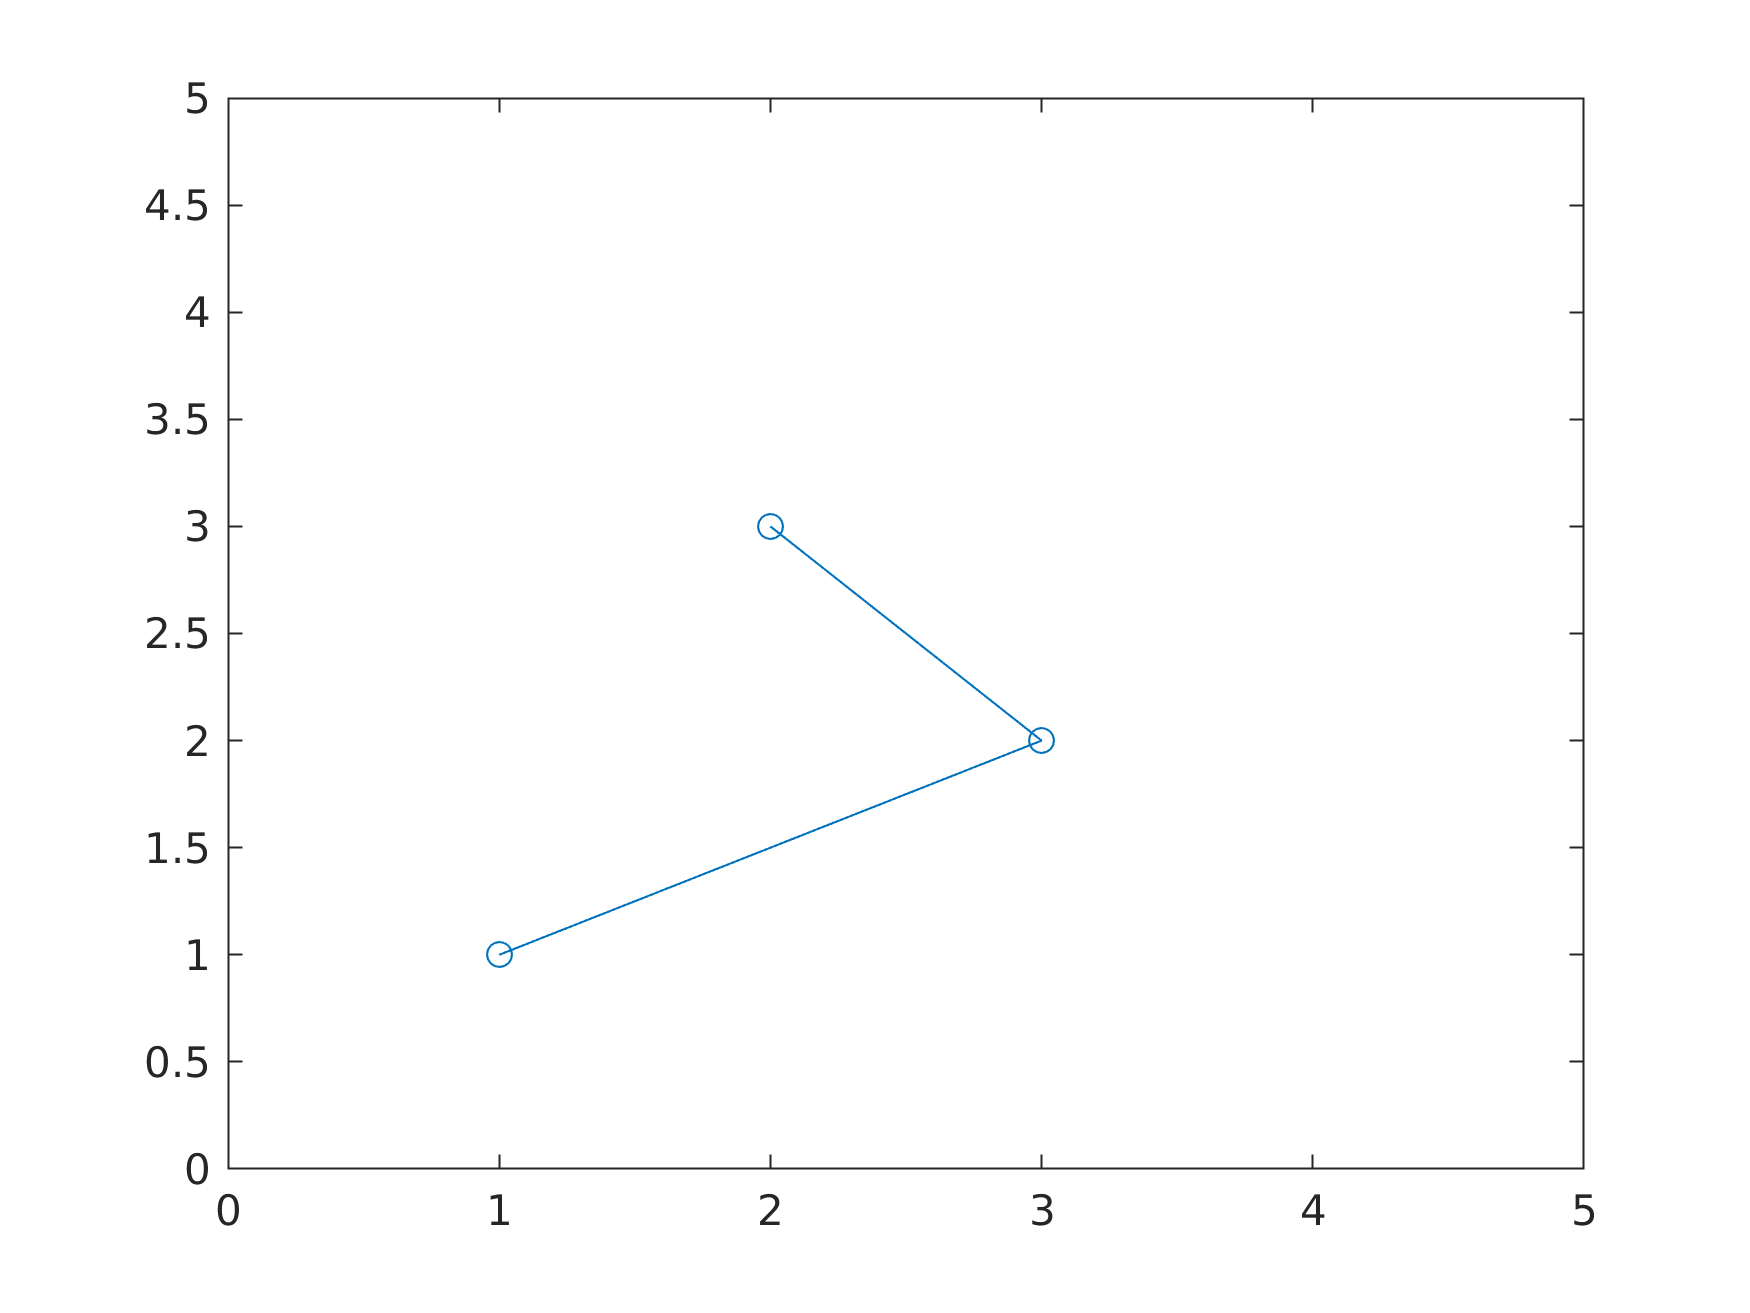
\includegraphics[width=8cm]{pic/basic_plotting_010.png}
\begin{hint}
The commands \verb!plot!, \verb!xlim! and \verb!ylim! can be useful.
\end{hint}
\begin{sol}
A solution is:
\begin{verbatim}
figure(1);
clf;
x = [1, 3, 2];
y = [1, 2, 3];
plot(x, y, '-o');
xlim([0, 5]);
ylim([0, 5]);
\end{verbatim}
\end{sol}
\end{ex}

\begin{ex}
Find a root of the function $f(x) = e^{-x} - x$.
\begin{hint}
The command \verb!fzero! can be useful.
\end{hint}
\begin{sol}
A solution is:
\begin{verbatim}
fh = @(x) exp(-x) - x
root1 = fzero(fh, 1)
\end{verbatim}
\end{sol}
\end{ex}

\begin{ex}
Find the minimum of the function $f(x) = e^x - 2x$.
\begin{hint}
The command \verb!fminsearch! can be useful.
\end{hint}
\begin{sol}
A solution is:
\begin{verbatim}
fh = @(x) -2x + exp(x);
fminsearch(fh, 1)
\end{verbatim}
\end{sol}
\end{ex}


\begin{ex}
Plot the functions $f(x) = e^x$ and $g(x) = 4x$ over the interval $x \in [-1, 3]$.
\begin{hint}
Define two function handles, one to each function.
Use the functions \verb!linspace!, \verb!hold on!, \verb!plot! and \verb!figure!.
\end{hint}
\begin{sol}
A solution is:
\begin{verbatim}
fh = @(x) exp(x);
gh = @(x) 4*x;
x = linspace(-1, 3);
figure(1);
clf;
hold on;
plot(x, fh(x));
plot(x, gh(x))
\end{verbatim}
\end{sol}
\end{ex}


\begin{ex}
Make the figure inserted below. Pay attention to the axes labels and the width of the plotted line. The visualized function is $f(x) = x^2 - x$. \par
\noindent
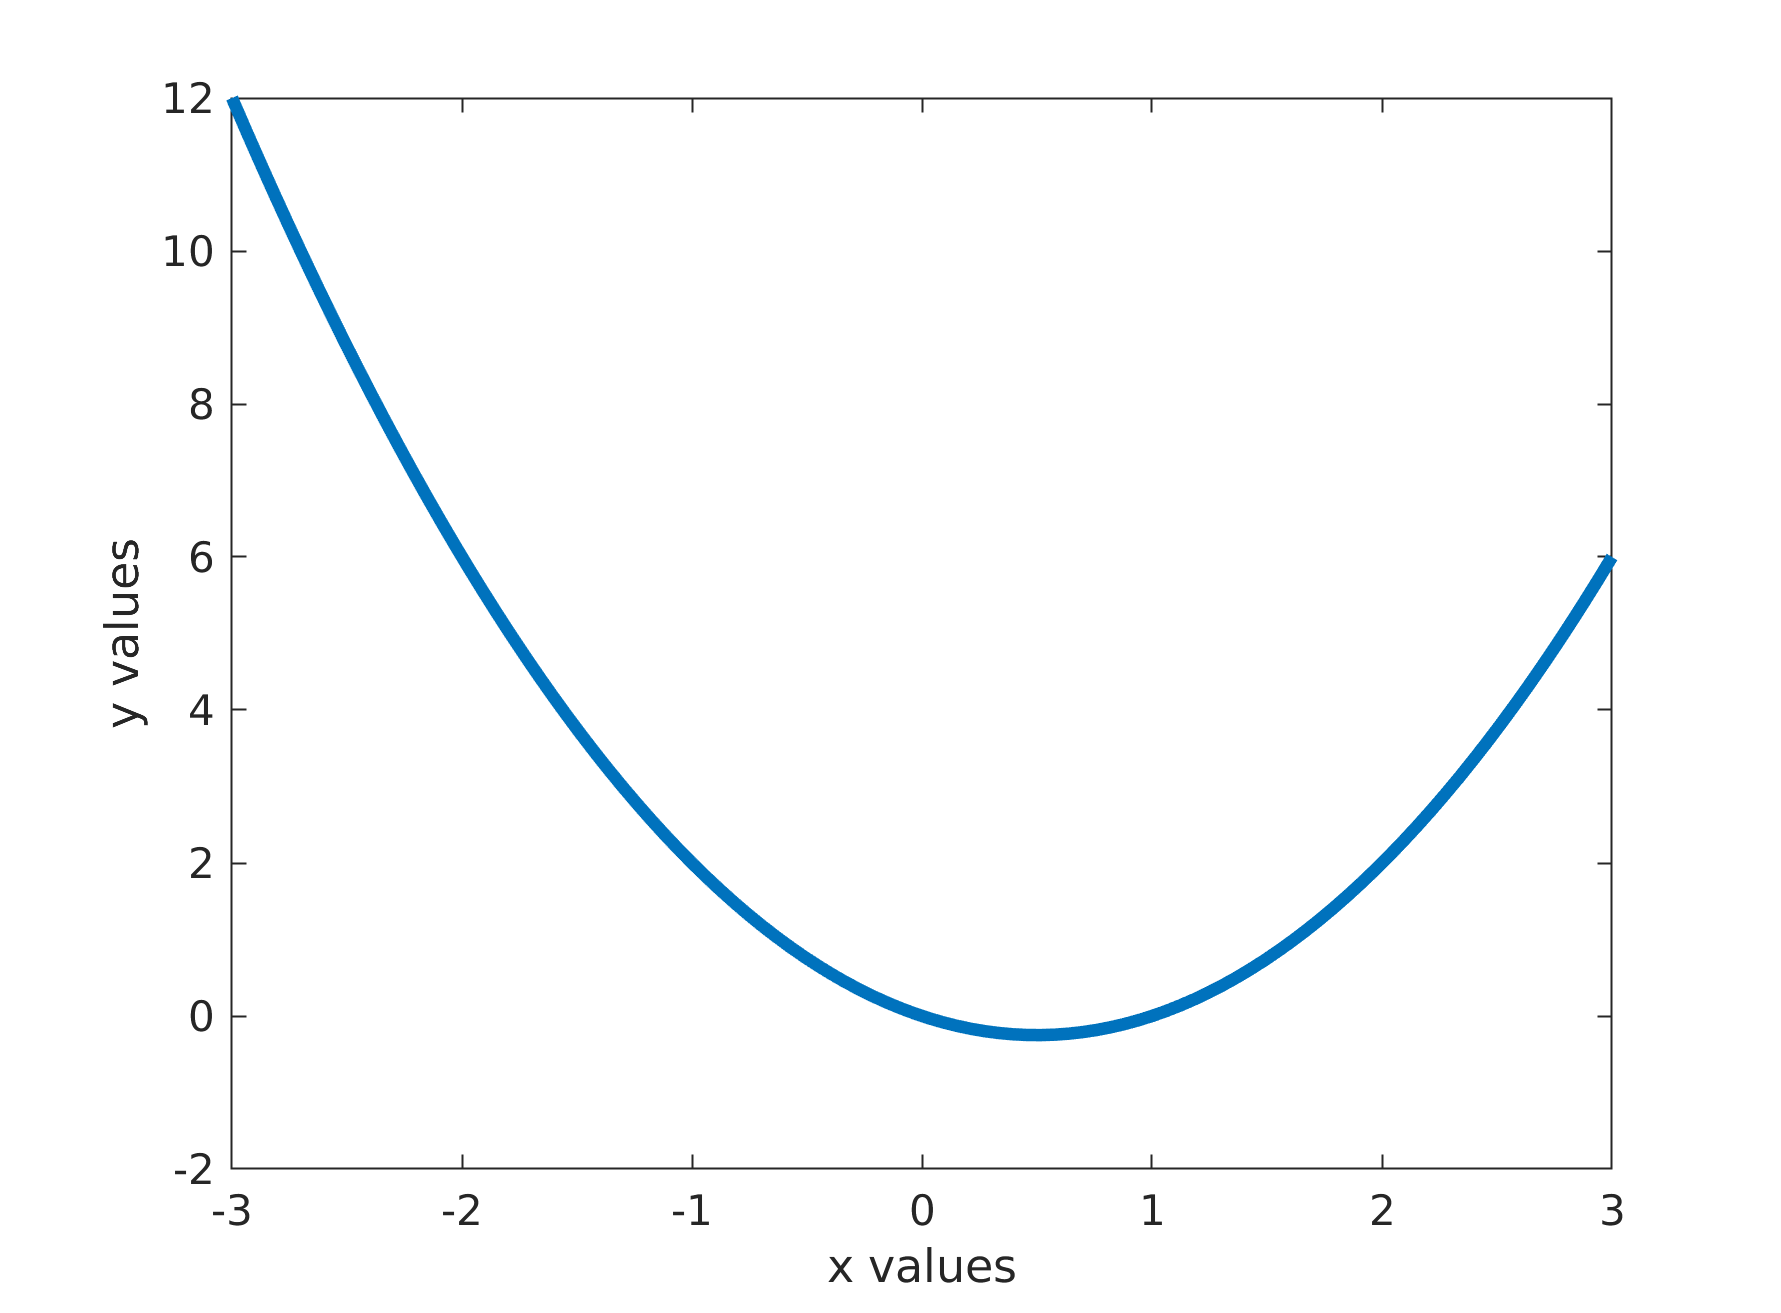
\includegraphics[width=8cm]{pic/basic_plotting_020.png}
\begin{hint}
The commands \verb!plot!, \verb!xlabel! and \verb!ylabel! can be useful.
\end{hint}
\begin{sol}
A solution is:
\begin{verbatim}
figure(1);
clf;
fh = @(x) -x + x.^2;
x = linspace(-3, 3);
plot(x, fh(x), 'LineWidth', 3);
xlabel('x values');
ylabel('y values');
\end{verbatim}
\end{sol}
\end{ex}


\begin{ex}
Find two numerical solutions to the equation
\[
e^{x} = 4x
\]
\begin{hint}
Write the equation on the form $f(x) = 0$ (collect all elements on the left hand side).
The command \verb!fzero! can be useful.
\end{hint}
\begin{sol}
A solution is:
\begin{verbatim}
fh = @(x) exp(x) - 4*x;
root1 = fzero(fh, 1)
root2 = fzero(fh, 3)
\end{verbatim}
\end{sol}
\end{ex}



\begin{ex}
Solve the set of linear equations
\begin{align*}
1	& = 5x + 2y	\\
0	& = -x + y + 3z + 2v	\\
-10 	& = x + 3y - 4z + v	\\
0	& = -2x + 3z - 2v 
\end{align*}
\begin{hint}
Write the system of equations on matrix form $A \cdot \vec{x} = \vec{b}$.
\end{hint}
\begin{sol}
A solution is:
\begin{verbatim}
A = [5, 2, 0, 0; -1, 1, 3, 2; 1, 3, -4, 1; -2, 0, 3, -2];
b = [1; 0; -10; 0];
x = linsolve(A, b)
A * x
\end{verbatim}
\end{sol}
\end{ex}



\begin{ex}
Enter\label{exPlotDataToFitLinearModelTo}
the following values for $x$ and $y$ and plot the points.
Then describe the trend you are observing in the data.
\begin{verbatim}
x = [1, 2, 3, 5];
y = [4, 3, 2, 1];
\end{verbatim}
\begin{hint}
Use the \verb!plot! method.
\end{hint}
\begin{sol}
A solution is:
\begin{verbatim}
x = [1, 2, 3, 5];
y = [4, 3, 2, 1];
figure(1);
clf;
plot(x, y, 'o');
\end{verbatim}
From the plot I see that the $y$ values decreases as the $x$ values increases.
\end{sol}
\end{ex}

\begin{ex}
This\label{exPlotDataToFitLinearModelTo2}
exercise is a continuation of exercise \ref{exPlotDataToFitLinearModelTo}.
Implement a linear model $y = a \cdot x + b$ in matlab. 
The linear model should be defined like below, where P is a vector containing the 
model parameters $a$ and $b$.
\begin{verbatim}
model = @(x, P) <fill in stuff here>;
\end{verbatim}
\begin{hint}
The output of the model should match the output below.
\begin{verbatim}
>> model([1, 2, 3, 5], [-1, 5])
ans =
     4     3     2     0
\end{verbatim}
\end{hint}
\begin{sol}
A solution is:
\begin{verbatim}
model = @(x, P) P(1) * x + P(2);
\end{verbatim}
\end{sol}
\end{ex}

\begin{ex}
This \label{exPlotDataToFitLinearModelTo3}
exercise is a continuation of exercise \ref{exPlotDataToFitLinearModelTo2}.
Implement a method that calculates the squared error
between the model and observations.
\[
\text{squared error} = \sum_i \left(y_i - \text{model}(x_i)\right)^2
\]
Assume that the $x$ and $y$ values are saved in the variables 
\verb!x! and \verb!y! respectively.
\begin{verbatim}
model_error = @(P) <fill in stuff here>;
\end{verbatim}
\begin{hint}
The \verb!sum! function is helpful.
\end{hint}
\begin{sol}
A solution is:
\begin{verbatim}
>> x = [1, 2, 3, 5];
>> y = [4, 3, 2, 1];
>> model = @(x, P) P(1) * x + P(2);
>> model_error = @(P) sum((y - model(x, P)).^2);
>> squared_error = model_error([-1.2, 5])
squared_error =
    4.5600
\end{verbatim}
\end{sol}
\end{ex}

\begin{ex}
This exercise is a continuation of exercise \ref{exPlotDataToFitLinearModelTo3}.
Minimize the squared error, defined in exercise \ref{exPlotDataToFitLinearModelTo3} and then plot the model with the 
found parameter values along with the original data.
\begin{hint}
The \verb!fminsearch! function is helpful, it should converge to 
the proper solution independent of the initial guess.
The solution contains the following values $-0.7429$ and $4.5429$.
\end{hint}
\begin{sol}
A solution is:
\begin{verbatim}
x = [1, 2, 3, 5];
y = [4, 3, 2, 1];
model = @(x, P) P(1) * x + P(2);
model_error = @(P) sum((y - model(x, P)).^2);
P = fminsearch(model_error, [4, 2])

xvals = linspace(0, 6);
figure(1);
clf;
hold on;
plot(x, y, 'o');
plot(xvals, model(xvals, P));
\end{verbatim}
\end{sol}
\end{ex}



\begin{ex}
Plot the three functions given below in the same plot.
\[
f(x) = \frac{1}{x + 1} \qquad \qquad g(x) = \frac{1}{x + 3} \qquad \qquad h(x) = \frac{1}{(x + 1)(x + 3)}
\]
Do the functions have something in common?
\begin{hint}
Look at the discontinuities of the functions. Where are they placed?
\end{hint}
\begin{sol}
A solution is:
\begin{verbatim}
fh = @(x) 1 ./ (x + 1);
gh = @(x) 1 ./ (x + 3);
hh = @(x) 1 ./ ((x + 1) .* (x + 3));
x = linspace(-5, 1, 1000);
figure(1);
clf; 
hold on;
plot(x, fh(x));
plot(x, gh(x));
plot(x, hh(x));
ylim([-4, 4]);
\end{verbatim}
\end{sol}
\end{ex}

\begin{ex}
Given the three functions below:
\[
f(x) = \frac{1}{x + 1} \qquad \qquad g(x) = \frac{1}{x + 3} \qquad \qquad h(x) = \frac{1}{(x + 1)(x + 3)}
\]
Plot $h(x)$ and a linear combination of $f(x)$ and $g(x)$ in the same plot.
Adjust the coefficients of $f(x)$ and $g(x)$, so that the two plotted functions 
becomes as similar as possible.
\begin{hint}
An example of a linear combination of $f(x)$ and $g(x)$ is
\[
2 \cdot f(x) + 3 \cdot g(x)
\]
\end{hint}
\begin{sol}
A solution is:
\begin{verbatim}
fh = @(x) 1 ./ (x + 1);
gh = @(x) 1 ./ (x + 3);
hh = @(x) 1 ./ ((x + 1) .* (x + 3));
figure(2);
clf; 
hold on;
plot(x, 0.5*fh(x) - 0.5*gh(x));
plot(x, hh(x), 'LineStyle', '- -', 'LineWidth', 3);
ylim([-4, 4]);
\end{verbatim}
\end{sol}
\end{ex}




\section{2019-10-24 Numerical integration}

\todo[inline]{Add exercises where some integration rules are tested using numerical methods (this should equal that, check using the integral method in Matlab).}


\begin{ex}[Reference value]%
Evaluate the integral below numerically using the \verb!integral! function.
\[
\int_0^5 e^{-x} \cdot \sin(x) dx
\]
\begin{hint}
The two first significant digits are 0.50.
\end{hint}
\begin{sol}
A solution is:
\begin{verbatim}
fh = @(x) exp(-x) .* sin(x);
integral(fh, 0, 5)
\end{verbatim}
\end{sol}
\end{ex}

\begin{ex}[Trapez rule]%
Evaluate \label{exTrapezRule}
the function:
\[
  e^{-x} \cdot \sin(x) dx
\]
at 10 evenly spread x-values from 0 to 5, the values in this list
will be called $x_i$ in the following.
Then calculate the sum
\[
\sum_{i = 1}^{9} \frac{x_i + x_{i + 1}}{2} \cdot (x_{i + 1} - x_i)
\]
\begin{hint}
Use \verb!linspace! to generate a list of x-values.
\end{hint}
\begin{sol}
A solution is:
\begin{lstlisting}
fh = @(x) exp(-x) .* sin(x);
nvals = 10;
x = linspace(0, 5, nvals);
fx = fh(x);
value = 0;
for k = 1:(nvals - 1)
    avg_height = 0.5*(fx(k) + fx(k + 1));
    dx = x(k + 1) - x(k);
    value = value + avg_height * dx;
end
\end{lstlisting}
\end{sol}
\end{ex}

\begin{ex}[Trapez rule as a function]%
Create a function that uses the Trapez rule to estimate the 
value of a definite integral.
The function must have the signature
\begin{lstlisting}
function res = trapez_rule(fh, x_low, x_high, n_intervals)
\end{lstlisting}
Use the following examples to test the function
\begin{lstlisting}
>> trapez_rule(fh, 0, 5, 10)
ans = 0.4770
>> trapez_rule(fh, 0, 5, 20)
ans = 0.4966
>> trapez_rule(fh, 0, 5, 100)
ans = 0.5021
\end{lstlisting}
\begin{hint}
Use your solution from exercise \ref{exTrapezRule} and build a function around it.
\end{hint}
\begin{sol}
A solution is:
\begin{lstlisting}
function res = trapez_rule(fh, x_low, x_high, n_intervals)

x = linspace(x_low, x_high, n_intervals);
fx = fh(x);
res = 0;
for k = 1:(n_intervals - 1)
    avg_height = 0.5*(fx(k) + fx(k + 1));
    dx = x(k + 1) - x(k);
    res = res + avg_height * dx;
end

end
\end{lstlisting}
\end{sol}
\end{ex}

\begin{ex}
Rewrite the following function such that it uses a for loop.

\begin{lstlisting}
function functionThatRepeatsStuff()
disp(1);
disp(1);
disp(1);
disp(1);
disp(1);
disp(1);
disp(1);
disp(1);
end
\end{lstlisting}
\begin{hint}
Identify what is repeated and how many times it is repeated.
\end{hint}
\begin{sol}
A solution is:
\begin{lstlisting}
function functionThatRepeatsStuff()
for k = 1:8
  disp(1);
end
end
\end{lstlisting}
\end{sol}
\end{ex}



\begin{ex}
Rewrite the following function such that it uses a for loop.
\begin{lstlisting}
function functionThatCounts()
disp(1);
disp(2);
disp(3);
disp(4);
disp(5);
disp(6);
disp(7);
disp(8);
disp(9);
end
\end{lstlisting}
\begin{hint}
Use a for loop, with a structure as shown here:
\begin{lstlisting}
for k = 1:4
end
\end{lstlisting}
\end{hint}
\begin{sol}
A solution is:
\begin{lstlisting}
function functionThatCounts()
for k = 1:9
  disp(k);
end
end
\end{lstlisting}
\end{sol}
\end{ex}



\begin{ex}
Create \label{exSumOfPositiveIntegersLessThanN}
a function that takes one positive integer, n, as argument and
calculates the sum of all integers in the range $1, 2, ..., n$.

\begin{lstlisting}
function res = sumOfIntegersLessThanOrEqualTo(n)
\end{lstlisting}
Example usage of the function:
\begin{lstlisting}
>> sumOfIntegersLessThanOrEqualTo(1);
>> sumOfIntegersLessThanOrEqualTo(1)
ans = 1
>> sumOfIntegersLessThanOrEqualTo(5)
ans = 15
>> sumOfIntegersLessThanOrEqualTo(10)
ans = 55
>> sumOfIntegersLessThanOrEqualTo(100)
ans = 5050
\end{lstlisting}
\begin{hint}
Use a for loop, with a structure as shown here:
\begin{lstlisting}
for k = 1:n
end
\end{lstlisting}
Prior to the for loop, create a variable and set its value to 0.
Then update the value in the variable for each cycle in the for loop.
\end{hint}
\begin{sol}
A solution is:
\begin{lstlisting}
function res = sumOfIntegersLessThanOrEqualTo(n)
res = 0;
for k = 1:n
  res = res + 1;
end
end
\end{lstlisting}
\end{sol}
\end{ex}




\begin{ex}
Create a function that takes one positive integer, n, as argument and
calculates the sum of all integers in the range $1, 2, ..., n$, which are even.

\begin{lstlisting}
function res = sumOfEvenIntegersLessThanOrEqualTo(n)
\end{lstlisting}
Example usage of the function:
\begin{lstlisting}
>> sumOfEvenIntegersLessThanOrEqualTo(1);
>> sumOfEvenIntegersLessThanOrEqualTo(1)
ans = 0
>> sumOfEvenIntegersLessThanOrEqualTo(5)
ans = 6
>> sumOfEvenIntegersLessThanOrEqualTo(10)
ans = 30
>> sumOfEvenIntegersLessThanOrEqualTo(100)
ans = 2550
\end{lstlisting}
\begin{hint}
Modify the solution to exercise \ref{exSumOfPositiveIntegersLessThanN}
so it only increments the variable when $k$ is even.
\end{hint}
\begin{sol}
A solution is:
\begin{lstlisting}
function res = sumOfEvenIntegersLessThanOrEqualTo(n)
res = 0;
for k = 1:n
  if(mod(k, 2) == 0)
    res = res + 1;
  end
end
end
\end{lstlisting}
\end{sol}
\end{ex}



\begin{ex}
Create a function that calculates the n'th Fibonacci number. The nth
fibonacci number can be calculated using the formula: 
\[
F_n = F_{n-1} + F_{n-2}
\]
with the two base cases $F_0 = 0$ and $F_1 = 1$. The sequence goes like
$0, 1, 1, 2, 3, 5, 8, 13, 21, 34, ...$

\begin{lstlisting}
function res = fib(n)
\end{lstlisting}
Example usage of the function:
\begin{lstlisting}
>> fib(0);
>> fib(0)
ans = 0
>> fib(1)
ans = 1
>> fib(6)
ans = 8
>> fib(17)
ans = 1597
>> fib(29)
ans = 514229
\end{lstlisting}
\begin{hint}
Use one or more if statements to ensure that the two base
cases are handled properly.
Then use the relation
\[
\textrm{fib}(n) = \textrm{fib}(n - 1) + \textrm{fib}(n - 2)
\]
\end{hint}
\begin{sol}
A solution is:
\begin{lstlisting}
function res = fib(n)

if(n < 2)
  res = n;
else
  res = fib(n - 1) + fib(n - 2);
end
end
\end{lstlisting}
\end{sol}
\end{ex}






\section{2019-11-04 Numerical solutions of differential equations}


\subsection{Euler's method}


\begin{ex}[Eulers method]%
Function definition:
\begin{lstlisting}
function [yvals, fcalls] = euler(fnc, xvals, y0)
% Uses the Euler method for approximating the first order
% differential equation defined by the function handle fnc.
%
% Input values:
% - fnc Function handle to a function which takes two
% input arguments and returns a scalar value.
% Eg. @(x, y) (y+sin(x))
% - xvals List of x values where the corresponding y
% values should be calculated.
% - y0 Initial state of the dependent function.
%
% Output values:
% - yvals Approximation of y(x) at the locations
% specified in xvals.
% - fcalls Number of function evaluations.
\end{lstlisting}
Example usage of the function:
\begin{lstlisting}
>> [yvals, fevals] = euler(@(x, y) y, [0:5], 1)
yvals =
1 2 4 8 16 32
fevals =
5
>> euler(@(x, y) y, [0:5], 2)
ans =
2 4 8 16 32 64
>> euler(@(x, y) 0.1*y, [0:5], 1)
ans =
1.0000 1.1000 1.2100 1.3310 1.4641 1.6105
>> euler(@(x, y) 0.1*y+0.2*x, [0:5], 1)
ans =
1.0000 1.1000 1.4100 1.9510 2.7461 3.8207
\end{lstlisting}
\begin{hint}
\end{hint}
\begin{sol}
A solution is:
\begin{lstlisting}
\end{lstlisting}
\end{sol}
\end{ex}

\begin{ex}
\label{excEulerConvergence} \\
For the initial value problem
\begin{align}
y'(t)
	& = 1.2 \cdot y(t) 	&
y(0) = 1
\end{align}
Determine the analytic solution and calculate the exact value of $y(3)$.
Use Euler's method to approximate $y(3)$ with different step lengths $h$.
How is the error related to the used step length?
\begin{hint}
\end{hint}
\begin{sol}
A solution is:
\begin{verbatim}
\end{verbatim}
\end{sol}
\end{ex}



\Closesolutionfile{hnt}
\Closesolutionfile{ans}


\newpage
\section{Hints}
\input{hints}


\newpage
\section{Solutions}
\input{ans}


\newpage
\section{Links to other resources}

Beginning Matlab Exercises, by R. J. Braun: 
\url{http://www.math.udel.edu/~braun/M349/Matlab_probs2.pdf}

\url{http://kom.aau.dk/~borre/matlab7/exercise.pdf}


\end{document}
